\documentclass{article}
\usepackage[utf8]{inputenc}
\usepackage{xeCJK}
\usepackage{enumitem}  % 引入 enumitem 宏包
\usepackage{graphicx} % 插入圖片的宏包
\usepackage{float} % 設置圖片浮動位置的宏包
\setCJKmainfont{Noto Serif CJK TC}

% \title{Multiple bibliographies with bibunits}

\usepackage{bibunits}
\usepackage[
	a4paper,
	left=1.2cm,
	right=1.2cm,
	top=1.5cm,
	bottom=1cm,
	nohead
]{geometry}

\begin{document}
\pagestyle{empty}  % 移除页码
\begin{bibunit}[plain]
\section{自传}
\subsection{基本背景}

我是黄柏曛,从小在台北长大,个性温柔大方,跟大陆学生或同事等都相处友好
,对任何新事物都有较强的学习驱动能力。
我高中毕业于台北市立中正高中,并在高中阶段就接触程序设计。
高中毕业后由于母亲是湖南人,中南大学又刚好在湖南,在家人的坚持下,
我选择前往大陆念书大学,并于2022毕业于中南大学计算机学院的软件工程。
2023年开始在中兴通讯担任IT软件工程师,深刻认识到自己的不足,
工作了两年后主动离职,下定决心要继续攻读硕士学位。

\subsection{培芽探索}
我还在念中正高中时有幸参加电脑老师开设的资讯程序的选修课程,一次的好奇与试
探,却对写程序产生兴趣,随后我一直利用课后时间与电脑老师交流,并利用宝贵的中休时
间亲自跑到电脑教室学习程序的编写。很幸运地那年刚好是台湾师范大学开放高中生的 C
语言程序选修的探索时间,电脑老师鼓励我们学生一起去选修课程,也是在这次机缘下认识
了蒋教授,教授的课程作业让我成长了很多,包括在编写程序的思维方式:先思考如何用最
笨的方式 AC,再进一步去减少时间复杂度与空间复杂度,让程序更有效运行。
我也在台师大选修程序语言的这段期间初次入门参加了 APCS 考试,我当时拿了 7
段,我还是很感谢这段经历,我也因此确定了未来方向:计算机科学与软件工程。

\subsection{培养动手能力}
在中南大学大一期间,除了加强了 C++、JAVA 基础还有 HTML 网页开发,虽然老师上课
的教材篇老旧,但我依然去 W3C 或是 MDN 去阅读文档。
大二期间我修了操作系统、数据库、资料结构、算法、计算机网络等课程更加深了对于计
算机方面的知识,也在大二频繁使用 Github 与同学之间完成网页开发课程项目,对于 Git
的使用也越来越熟练。开发网页项目一开始是使用 SpringMVC 编写 JSP 页面实现宠物商店,
资料存储使用 MySQL,我主力负责 frontend 设计,不仅学会了 jQuery 框架、Bootstrap 框
架,也熟悉掌握了 HTTP 的请求。在之后使用 VueJs 和 SpringBoot+MyBatis 去重构项目。
大三也因为个人兴趣选修了软件测试、机器学习与资料探勘、电子商务、软件体系结构(JAVA
设计模式)、云计算及应用等探索式的课程。这些加强了我对于未来发展方向的认知。

\subsection{大学科研与竞赛}
从大一开始我就踊跃参加各大比赛,全国大学生创新创业训练分别获得过一次校级评定、两次省级评定。
2020年与同学跨科系组队参加交通科技运输大赛获得校级一等奖,
并于2021年与商学院学生跨院系参加全国大学生电子商务“创新、创意及创业”挑战赛获校级二等奖。
大四毕业论文以“基于状态检测的网关优化与可视化”的工业物联网相关实务类型为主题获评定为优等毕业论文。

\subsection{自主学习与交流}
课外我不仅自主学会了目前主流的 VueJs、Angular 等框架(主要学习 MVVM 架构),并且
学习 Python Flask 微服务框架、Golang 的 WebSocket 聊天室、SpringBoot 框架,除此之
外自己在 Server 上使用 Nginx Web Server 部署网页,了解到 Nginx 在各服务器集群的负
载均衡配置和配置端口反向代理。因为我在 Telegram 通讯软件群组中因为督促大家英文打
卡,所以自己利用开源库编写了一个 TG 多群组成员每日英文打卡 Bot。
大学期间,我就有自己用 Github Page 和 Hugo 搭建自己的 Blog,并且玩起了 ArchLinux
等更多自定义化 Linux 发行版,在 ArchLinux CN 社群讨论技术问题。我也善用 StackOver-
flow、Github PR ISSUE 去跟其他开发者沟通交流。

\subsection{校外实习与工作经验}
到了大四,我因为想要在企业中有一份属于自己的成长,一个人到了上海的工业物联网公司
进行嵌入式应用研发,在一开始熟悉了公司的嵌入式物联网网关。对于嵌入式网关的开发,
因为面对有 Moxa、ORing、大全赛雪龙等客户需求,我需要为他们开发物联网的嵌入式应
用,包括使用 Modbus RTU/TCP 协议透过 RS-485 串列埠传输指令、使用 FTP 协议传输物
联网装置报错日志、透过串口转网口传输温度、GPIO PIN 脚位控制 Beeper 和 DIP 等。最
后主力研发全新的嵌入式网页控制,取代公司旧版的嵌入式网页。
即使毕业后回到台湾的期间,也趁着闲暇做起的软件外包,包括基于Angular的Android
应用和嵌入式应用控制GPIO。

入职中兴通讯后,我在架构团队快速学习敏捷开发模式与团队之间协同,在每次迭代开发期间
与团队协作完成一个又一个待交付需求。我负责运维工作、
项目组开发工作和架构部门的整体事项,在这些工作中也极大锻炼了我的个人沟通表达能力、
需求与设计文档理解能力和解决问题的能力。

\end{bibunit}


\begin{bibunit}[alpha]
\section{攻读研究生阶段的学习计划}

\subsection{研究生期间}
\subsubsection{研一阶段}

\begin{itemize}[parsep=0.5ex]
	\item 了解毕业要求,需要发表多少论文以及哪个等级的论文;
	\item 每周保持论文的阅读量,并在实验室的例会中轮流分享自己科研进度,锻炼自己的表达能力;
	\item 平时阅读文献期间,纪录可能有机会做得更好且加以改进后能发表的论文主题;
	\item 学习分布式系统基础,动手搭建一套系统,深入了解Kubernetes集群和云原生;
	\item 练习编写设计软件架构设计文档和详细设计文档;
	\item 熟练使用数据可视化工具MATLAB;
	\item 学习演化式算法,认知到多目标最佳化与机器学习。
	\end{itemize}
	
	\subsubsection{研二阶段}
	\begin{itemize}[parsep=0.5ex]
	\item 多和导师沟通并确定毕业论文方向,开始撰写毕业论文开题报告;
	\item 每周持续阅读论文期刊,并撰写1-2篇小论文,准备论文投稿;
	\item 学习SaaS软件交付模型和PaaS云服务模型;
	\item 为实验室针对实验室网络资源构建NAS服务器环境,帮助实验室的开发项目和论文资料的共享;
	\item 学习大模型应用,并思考如何结合在不同领域;
	\item 积极申请担任助教的机会。
	\end{itemize}
	
	\subsubsection{研三阶段}
	
	\begin{itemize}[parsep=0.5ex]
	\item 学习分散式数据库与资料备份算法策略,避免数据库占用记忆体,保证数据库的资料完整性;
	\item 参与开源活动、前沿技术讲座或企业技术分享会;
	\item 开始寻找实习机会,把握机会能在寒暑假外出企业实习;
	\item 完成毕业论文,修改、润色、去重,达到毕业要求;
	\end{itemize}

\subsection{毕业后}

\begin{itemize}[parsep=0.5ex]
\item 与实验室的同学们保持联系,互相分享业内前沿知识;
\item 规划是否留美深造或留美工作。
\end{itemize}

\end{bibunit}

\begin{bibunit}[alpha]
	\section{报考动机}
	经历过大学的洗礼与成长,我对于写程序项目这件事就像搭积木一样,要先有一份设计图,
	再进行合作与需求讨论,我认为成功的项目是需要具备一个完整与相对合理的架构,能
	达到多模块解耦合独立运行。对我来说,程序语言在其中就像一实现工具,
	核心的思想还是找到问题并解决问题。

	\begin{figure}[htbp]
		\centering
		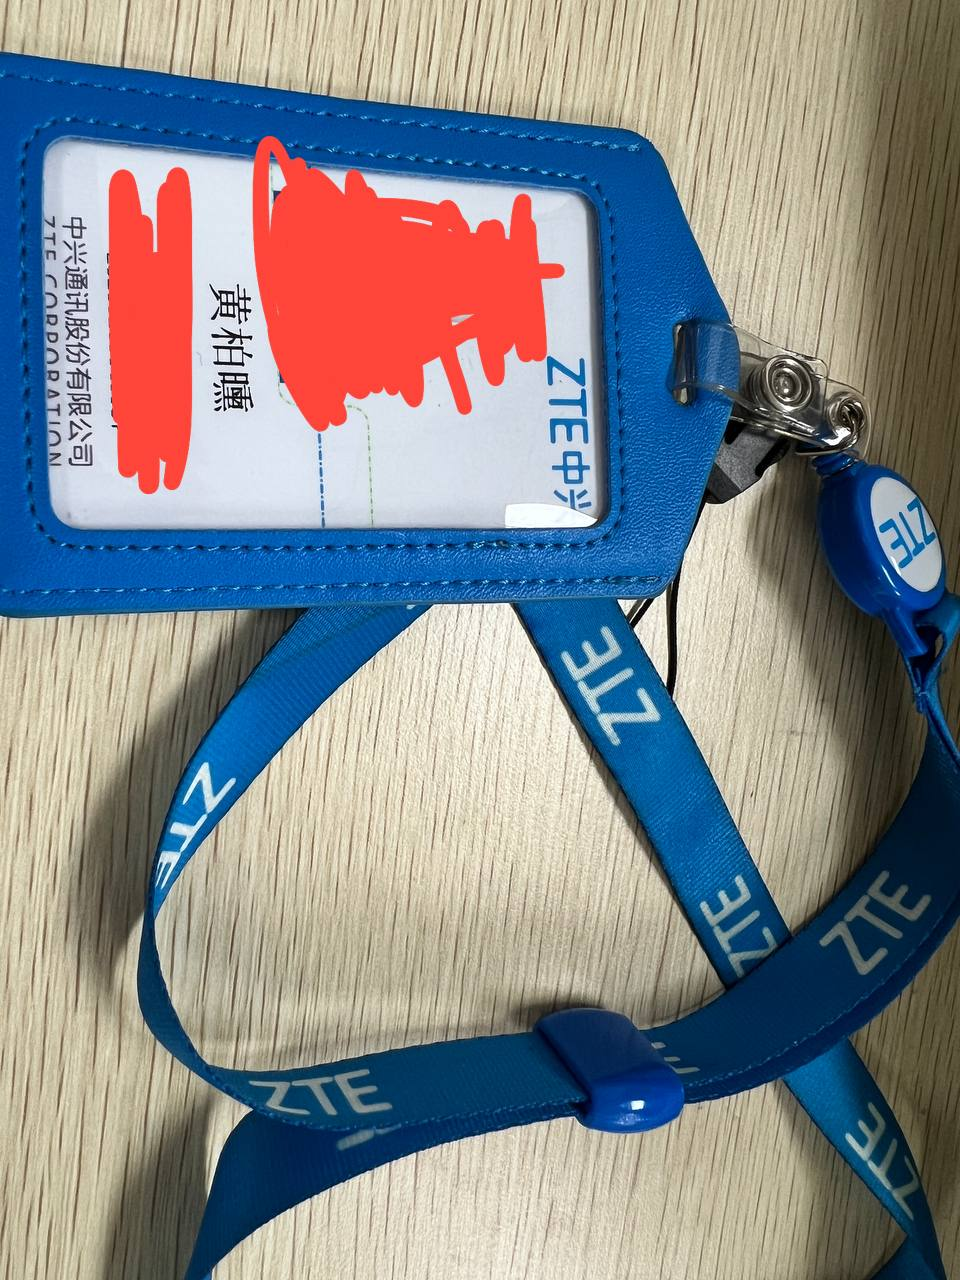
\includegraphics[angle=90, width=0.5\textwidth]{./img/work_carkd.jpg}  % 旋转图片90度
		\caption{任职于中兴通讯时的工卡}
		\label{fig:workCard}
	\end{figure}

	我在中兴通讯工作两年后,我成为团队和项目组的主力开发。
	第一年我在工作中,我完整参与了使用Langchain框架调用llm自动化生成项目的UT代码,最终团队获得公司大部门AI提效一等奖,并应用在实际开发流程中。此时我还停留在应用层面。
	然而在第二年,我成为AI新闻摘要智能体的主力前端和后端协助,在此期间负责Agent前端的所有设计、
	搭建后端项目结构,在这个项目中我感觉到我更想在科研领域上有所作为的热情,
	我想要深入了解AI,并实际应用在特定领域进行提效,而不是停留在应用框架的层面。
	一段时间的沉淀后,我决定继续深造自己。

	我希望在读研阶段形成自己的方法论,锻炼自己解决问题能力,进一步影响到我的思维模式,
	并在每次的科研实验中提炼出自己的核心观点和实验价值,不仅为科研做出贡献也提升自己的表达能力。
	\putbib[refs2]
\end{bibunit}



\end{document}

